% The restriction setup: 𝔓 above 𝔭 above (p) in the tower L/K/ℚ,
% with Frobenius elements upstairs and downstairs.
% Source: book/tex/alg-NT/frobenius.tex (§ Frobenius elements behave
% well with restriction) — tikzcd.
\documentclass[border=2mm]{standalone}
\usepackage{tikz}
\usetikzlibrary{arrows.meta}
\usepackage{amssymb}
\usepackage{amsmath}
\begin{document}
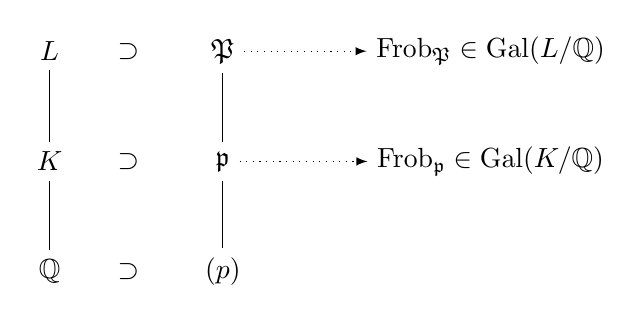
\begin{tikzpicture}[>=latex]
  \node (L)  at (0,2.8)   {$L$};
  \node (K)  at (0,1.4)   {$K$};
  \node (Q)  at (0,0)     {$\mathbb{Q}$};
  \node (s1) at (1.0,2.8) {$\supset$};
  \node (s2) at (1.0,1.4) {$\supset$};
  \node (s3) at (1.0,0)   {$\supset$};
  \node (PP) at (2.2,2.8) {$\mathfrak{P}$};
  \node (pp) at (2.2,1.4) {$\mathfrak{p}$};
  \node (p)  at (2.2,0)   {$(p)$};
  \node (FL) at (5.6,2.8) {$\operatorname{Frob}_{\mathfrak{P}} \in \operatorname{Gal}(L/\mathbb{Q})$};
  \node (FK) at (5.6,1.4) {$\operatorname{Frob}_{\mathfrak{p}} \in \operatorname{Gal}(K/\mathbb{Q})$};
  \draw (L) -- (K) -- (Q);
  \draw (PP) -- (pp) -- (p);
  \draw[dotted, ->] (PP) -- (FL);
  \draw[dotted, ->] (pp) -- (FK);
\end{tikzpicture}
\end{document}
